\documentclass[11pt]{article}

\usepackage[a4paper,margin=1in]{geometry}
\usepackage{amsmath,amssymb,amsthm}
\usepackage{graphicx}
\usepackage{tikz}
\usepackage{hyperref}
\usepackage{enumitem}
\usepackage{booktabs}
\usepackage{float}

\title{
Orthogonal Dual-Tree Topologies for Fault-Tolerant Distributed Aggregation
}

\author{
Dada Khalandhar Gooty
}

\date{\today}

\begin{document}

\maketitle

\begin{abstract}

Tree-based communication topologies are widely used in distributed machine learning and distributed aggregation systems due to their logarithmic communication depth and efficient hierarchical structure. However, conventional tree topologies suffer from poor fault tolerance because failure of an internal node disconnects entire dependent subtrees.

This work proposes a preliminary communication topology based on two complementary spanning trees constructed over the same logical node set. The proposed design attempts to reduce persistent node criticality by assigning complementary hierarchical roles across the two trees. Nodes that are highly critical in one tree are intentionally placed in lower-criticality positions in the second tree.

Unlike conventional redundant tree approaches, this work additionally introduces explicit inter-tree identity connections between corresponding node instances across the two trees. This layered dual-tree structure enables alternate routing paths while preserving hierarchical communication efficiency.

This document presents the preliminary formulation, intuition, structural definitions, and initial theoretical direction of the proposed topology.

\end{abstract}

\section{Introduction}

Distributed machine learning systems commonly employ hierarchical communication structures for operations such as:

\begin{itemize}
    \item gradient aggregation,
    \item parameter synchronization,
    \item reduce and all-reduce operations,
    \item hierarchical broadcast.
\end{itemize}

Tree-based communication structures are attractive because they provide:

\begin{itemize}
    \item logarithmic communication depth,
    \item scalable aggregation,
    \item low communication overhead.
\end{itemize}

However, conventional trees suffer from a major limitation:

\begin{quote}
Failure of an internal node disconnects all dependent descendants.
\end{quote}

This creates a significant reliability issue for large-scale distributed systems and distributed machine learning workloads.

This work proposes a preliminary dual-tree topology intended to reduce such failure sensitivity.

\section{Layered Dual-Tree Topology}

Let:

\[
V = \{v_1,v_2,\dots,v_n\}
\]

be the logical node set.

Two tree layers are constructed:

\[
T_1 = (V_1,E_1)
\]

\[
T_2 = (V_2,E_2)
\]

where:

\[
V_1 = \{v_1^{(1)},v_2^{(1)},\dots,v_n^{(1)}\}
\]

\[
V_2 = \{v_1^{(2)},v_2^{(2)},\dots,v_n^{(2)}\}
\]

represent node instances in Tree 1 and Tree 2 respectively.

\subsection{Inter-Tree Identity Connections}

For every logical node \(v_i\), an explicit inter-tree connection is introduced between its two layer instances:

\[
E_c =
\{
(v_i^{(1)},v_i^{(2)})
\mid
1 \le i \le n
\}
\]

These edges represent identity-preserving transitions between the two trees.

The complete communication graph is therefore:

\[
G =
(V_1 \cup V_2,
E_1 \cup E_2 \cup E_c)
\]

This formulation converts the topology into a layered redundant communication graph rather than a conventional single-tree hierarchy.

\section{Core Design Principle}

The central idea of the proposed topology is:

\begin{quote}
Node criticality should be anti-correlated across the two trees.
\end{quote}

Informally:

\begin{itemize}
    \item Nodes highly critical in \(T_1\) should become minimally critical in \(T_2\).
    \item Nodes near the periphery of \(T_1\) should become structurally important in \(T_2\).
\end{itemize}

This attempts to avoid persistent bottleneck nodes across the combined communication structure.

\subsection{Initial Role-Inversion Intuition}

An initial motivating intuition is:

\[
L(T_1) \approx I(T_2)
\]

\[
I(T_1) \approx L(T_2)
\]

where:

\begin{itemize}
    \item \(L(T)\) denotes leaf nodes,
    \item \(I(T)\) denotes internal nodes.
\end{itemize}

Exact inversion may not always be feasible under strict binary tree constraints. Therefore, approximate inversion or criticality inversion becomes the practical design objective.

\section{Node Criticality}

Define a node criticality function:

\[
C(v,T)
\]

which measures the structural importance of node \(v\) within tree \(T\).

Possible definitions include:

\begin{itemize}
    \item subtree size,
    \item betweenness centrality,
    \item ancestor dependency count,
    \item distance from root.
\end{itemize}

The proposed topology seeks to minimize persistent criticality across both trees.

A preliminary objective function is:

\[
\sum_{v \in V}
C(v,T_1)C(v,T_2)
\]

Minimizing this objective discourages nodes from simultaneously becoming highly critical in both trees.

\section{Structural Diversity}

Fault tolerance depends not only on redundancy, but also on structural diversity between the trees.

The proposed topology therefore attempts to minimize overlap between:

\begin{itemize}
    \item ancestor relationships,
    \item articulation structures,
    \item routing dependencies,
    \item communication bottlenecks.
\end{itemize}

The intention is that local failures in one tree become non-local in the second tree.

\section{Fault-Tolerance Intuition}

Consider failure of an internal node in \(T_1\).

In a conventional tree:

\begin{itemize}
    \item all descendants become disconnected.
\end{itemize}

In the proposed dual-tree structure:

\begin{itemize}
    \item descendants may transition through inter-tree identity edges,
    \item reroute through alternate dependency structures in \(T_2\),
    \item and potentially reconnect through unaffected regions of the communication graph.
\end{itemize}

Thus the combined layered graph may remain connected even after single-node failures.

\section{Failure Model}

A logical node failure is assumed to remove both layer instances of the node:

\[
v_i^{(1)}
\]

and

\[
v_i^{(2)}
\]

simultaneously.

Thus failures represent physical node failures rather than isolated layer failures.

The topology attempts to maintain communication despite such coupled failures by ensuring dependency diversity across the two trees.

\section{Preliminary Theoretical Direction}

A central research question is whether the combined graph:

\[
G =
(V_1 \cup V_2,
E_1 \cup E_2 \cup E_c)
\]

can satisfy:

\[
\kappa(G)\ge2
\]

where:

\begin{itemize}
    \item \(\kappa(G)\) denotes graph vertex connectivity.
\end{itemize}

If true, the topology would remain connected after removal of any single logical node.

A preliminary conjecture is:

\begin{quote}
If the two trees maintain sufficiently distinct dependency structures and anti-correlated node criticality, then the combined graph may achieve improved fault tolerance compared to conventional tree topologies.
\end{quote}

Formal proof and exact construction conditions remain open problems.

\section{Illustrative Example}

Figure~\ref{fig:dual_tree} illustrates the conceptual layered dual-tree structure.

\begin{figure}[H]

\centering

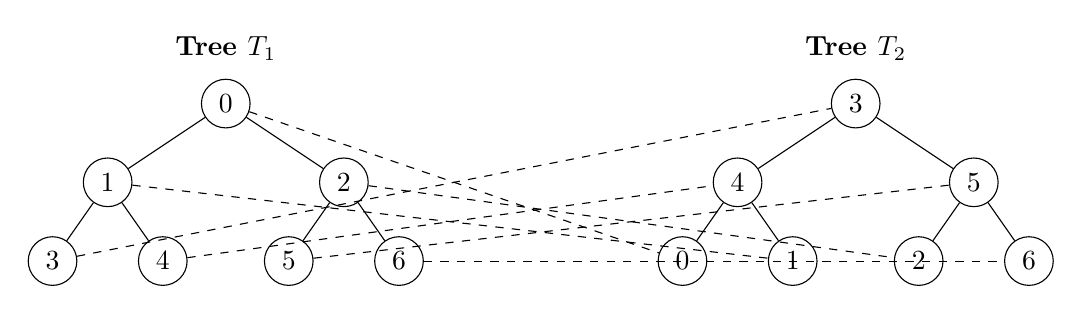
\begin{tikzpicture}[scale=1]

% ---------------- TREE 1 ----------------

\node[circle,draw] (A0) at (0,4) {0};
\node[circle,draw] (A1) at (-1.5,3) {1};
\node[circle,draw] (A2) at (1.5,3) {2};

\node[circle,draw] (A3) at (-2.2,2) {3};
\node[circle,draw] (A4) at (-0.8,2) {4};
\node[circle,draw] (A5) at (0.8,2) {5};
\node[circle,draw] (A6) at (2.2,2) {6};

\draw (A0)--(A1);
\draw (A0)--(A2);
\draw (A1)--(A3);
\draw (A1)--(A4);
\draw (A2)--(A5);
\draw (A2)--(A6);

\node at (0,4.7) {\textbf{Tree $T_1$}};

% ---------------- TREE 2 ----------------

\node[circle,draw] (B3) at (8,4) {3};
\node[circle,draw] (B4) at (6.5,3) {4};
\node[circle,draw] (B5) at (9.5,3) {5};

\node[circle,draw] (B0) at (5.8,2) {0};
\node[circle,draw] (B1) at (7.2,2) {1};
\node[circle,draw] (B2) at (8.8,2) {2};
\node[circle,draw] (B6) at (10.2,2) {6};

\draw (B3)--(B4);
\draw (B3)--(B5);
\draw (B4)--(B0);
\draw (B4)--(B1);
\draw (B5)--(B2);
\draw (B5)--(B6);

\node at (8,4.7) {\textbf{Tree $T_2$}};

% ---------------- INTER TREE CONNECTIONS ----------------

\draw[dashed] (A0)--(B0);
\draw[dashed] (A1)--(B1);
\draw[dashed] (A2)--(B2);
\draw[dashed] (A3)--(B3);
\draw[dashed] (A4)--(B4);
\draw[dashed] (A5)--(B5);
\draw[dashed] (A6)--(B6);

\end{tikzpicture}

\caption{
Conceptual layered dual-tree topology with explicit inter-tree identity connections.
Dashed lines represent inter-tree transitions between corresponding node instances.
}

\label{fig:dual_tree}

\end{figure}

\section{Potential Applications}

Potential applications include:

\begin{itemize}
    \item distributed machine learning,
    \item hierarchical aggregation,
    \item fault-tolerant overlays,
    \item distributed consensus,
    \item resilient communication fabrics.
\end{itemize}

\section{Open Problems}

Several important problems remain open:

\begin{itemize}
    \item optimal dual-tree construction algorithms,
    \item formal connectivity proofs,
    \item minimal-overlap hierarchy generation,
    \item communication latency analysis,
    \item dynamic rerouting algorithms,
    \item comparison with ring and fat-tree topologies,
    \item resilience under multiple simultaneous failures.
\end{itemize}

\section{Conclusion}

This work introduced a preliminary layered dual-tree communication topology intended to improve fault tolerance in hierarchical distributed systems.

The key idea is the construction of complementary spanning trees with anti-correlated node criticality and explicit inter-tree identity connections, reducing persistent bottlenecks and improving alternate communication path availability.

The proposed topology remains an early-stage research direction. Future work includes formal graph-theoretic analysis, construction algorithms, simulations, and distributed machine learning evaluation.

\bibliographystyle{plain}

\begin{thebibliography}{9}

\bibitem{graph}
Douglas B. West,
\textit{Introduction to Graph Theory},
Prentice Hall.

\bibitem{distributed}
Ian Foster,
\textit{Designing and Building Parallel Programs}.

\bibitem{fault}
George Karypis and Vipin Kumar,
``Fault-Tolerant Communication Topologies in Distributed Systems.''

\end{thebibliography}

\end{document}
